\documentclass{beamer}

\usepackage{setspace}
\usepackage{wrapfig}
\usepackage[utf8]{inputenc}
\usepackage[italian]{babel}
\usepackage{amsmath}
\usepackage{amsfonts}
\usepackage{amssymb}
\usepackage{graphicx}
\usepackage{listings}
\usepackage{pxfonts}

\lstset{language=C,basicstyle=\ttfamily\scriptsize,
                keywordstyle=\color{blue},
				identifierstyle=\bfseries,
                stringstyle=\color{red},
                commentstyle=\color{blue},
}

%\usetheme{Berkeley}
\usetheme{Goettingen}
\setbeamercovered{transparent} 
\setbeamertemplate{navigation symbols}{} 
%\useoutertheme[left]{sidebar}
%\usecolortheme{orchid}


\setbeamertemplate{footline}{\leavevmode\hbox{%
  \begin{beamercolorbox}%
  [wd=0.99\paperwidth,ht=6.1ex,right]%
  {author in head/foot}
  \usebeamerfont{title in head/foot}
    \vskip2pt\mbox{}
      \footnotesize{\insertframenumber\,/\,\inserttotalframenumber}
    \vskip3.5pt
  \end{beamercolorbox}}%
\vskip0pt}


\title
	{Heat Equation}
\author
	{Francesco Pasa\\
	 Enrico Panontin}
	
\institute{
	Technische Universität München\\ 
	Physics Department\\
	Parallelisation of Physics Calculations on GPUs with CUDA} 
\date{16 Juni 2016} 
\subject{}

\begin{document}
% 	titolo 
\begin{frame}
\maketitle
\end{frame}

% indice
\begin{frame}
\tableofcontents
\end{frame}

\section{Heat Equation}
%Theoretical introduction
\begin{frame}
\frametitle{Demonstration}
%\vspace{-20pt}
We consider heat propagation in a medium (e.g. a solid) far away from any state transition and we define:
\begin{description}
	\item[$\epsilon$]: internal energy density
	\item[$c$]: specific heat
	\item[$\rho$]: mass density
	\item[$T$]: temperature
\end{description}
By virtue of the first thermodinamic principle ($\Delta U = \Delta Q - L = \Delta Q$):
\begin{equation}\label{eq:first}
	d 
	\left[ 
		\int_\Omega 
		\! c \rho T  
		\, \mathrm{d}V
	\right]
	= 
	\left[
		- \int_{\partial \Omega} 
		\! \vec{J} \cdot \vec{n}
		\, \mathrm{d}S
	\right]
	\mathrm{d}t
\end{equation}
\end{frame}

\begin{frame}
\frametitle{Demonstration}
%\vspace{-20pt}
$$
	d 
	\left[ 
		\int_\Omega 
		\! c \rho T  
		\, \mathrm{d}V
	\right]
	= 
	\left[
		- \int_{\partial \Omega} 
		\! \vec{J} \cdot \vec{n}
		\, \mathrm{d}S
	\right]
	\mathrm{d}t
$$

{\it Newton-Fourier Law}, heat spreads and temperature becomes uniform throughout the medium:
\begin{equation}\label{eq:newton}
	\vec{J} = - k \vec{\nabla} T
\end{equation}

By substituting equation (\ref{eq:newton}) in (\ref{eq:first}) and applying the {\it divergence theorem} one gets the {\bf heat equation}:
\begin{equation}
	\frac
		{\partial T}
		{\partial t}
	- \frac{k}{c \rho}
	  \Delta T
	=0
\end{equation}
\end{frame}

\begin{frame}
\frametitle{Heat Equation}
$$
	\frac
		{\partial T}
		{\partial t}
	- \frac{k}{c \rho}
	  \Delta T
	= f(\vec{x}, t)
$$
\begin{itemize}
	\item First order in time
	\item Second order in space
	\item If we consider a heating system, we must add $f(\vec{x}, t)$
\end{itemize}
\end{frame}

\begin{frame}
\frametitle{Numerical Solution}
$$
	\frac
		{\partial T}
		{\partial t}
	- \frac{k}{c \rho}
	  \Delta T
	= f(\vec{x}, t)
$$

Discretize space and time: foreward difference for time, central difference for space:

\begin{equation}
	T_{i,j}^{n+1} = 
				T_{i,j}^n
				+ \eta
					\left[ T_{i+1,j}^n + T_{i-1,j}^n 
						 + T_{i,j+1}^n + T_{i,j-1}^n
						 - 4 T_{i,j}^n
					\right]
\end{equation}
where $n$ is the time index, $i,j$ are x-index and y-index, $\eta = \frac{k \Delta t}{c \rho (\Delta x)^2}$.
\end{frame}

\section{Our Code}
\begin{frame}
\frametitle{General Structure}
\begin{center}
	sim2d.cu

	\vspace{5mm}
	integrator.h
	
	integrator.cu
	\vspace{5mm}
	
	gl\_helper.cu
	
	gl\_helper.h
\end{center}
\end{frame}

\begin{frame}[fragile]
\frametitle{sim2d.cu}
Set: number of block, number of threads, other parameters.
\vspace{10mm}
\begin{lstlisting}
void readTiff(char *filename, float **raster, unsigned *w, 
		unsigned *h, float scale)
void step()

glutMainLoop()
\end{lstlisting}
\end{frame}

\begin{frame}[fragile]
\frametitle{integrator.cu}
\begin{lstlisting}
__global__ 
void stepSimulation2D(float *T, float *K, float *dT, 
			unsigned n_loop, uchar4 *tex, 
			char copy_tex)
__device__ 
void loadSharedMemory2D(const UsefulConstants consts, 
			float *T)
__device__ 
void integrate2D(const UsefulConstants consts, float *T, 
			float *K, float *dT)
\end{lstlisting}
\end{frame}

\begin{frame}[fragile]
\frametitle{loadSharedMemory2D}
\begin{lstlisting}
for (i = 0; i < n_loop; ++i) {
	local_T[lid_1d + i] = T[gid_1d + i];
	//d_operation[gid_1d+i] = 255;
}
__syncthreads();
\end{lstlisting}
\end{frame}

\begin{frame}[fragile]
\frametitle{loadSharedMemory2D}
\begin{center}
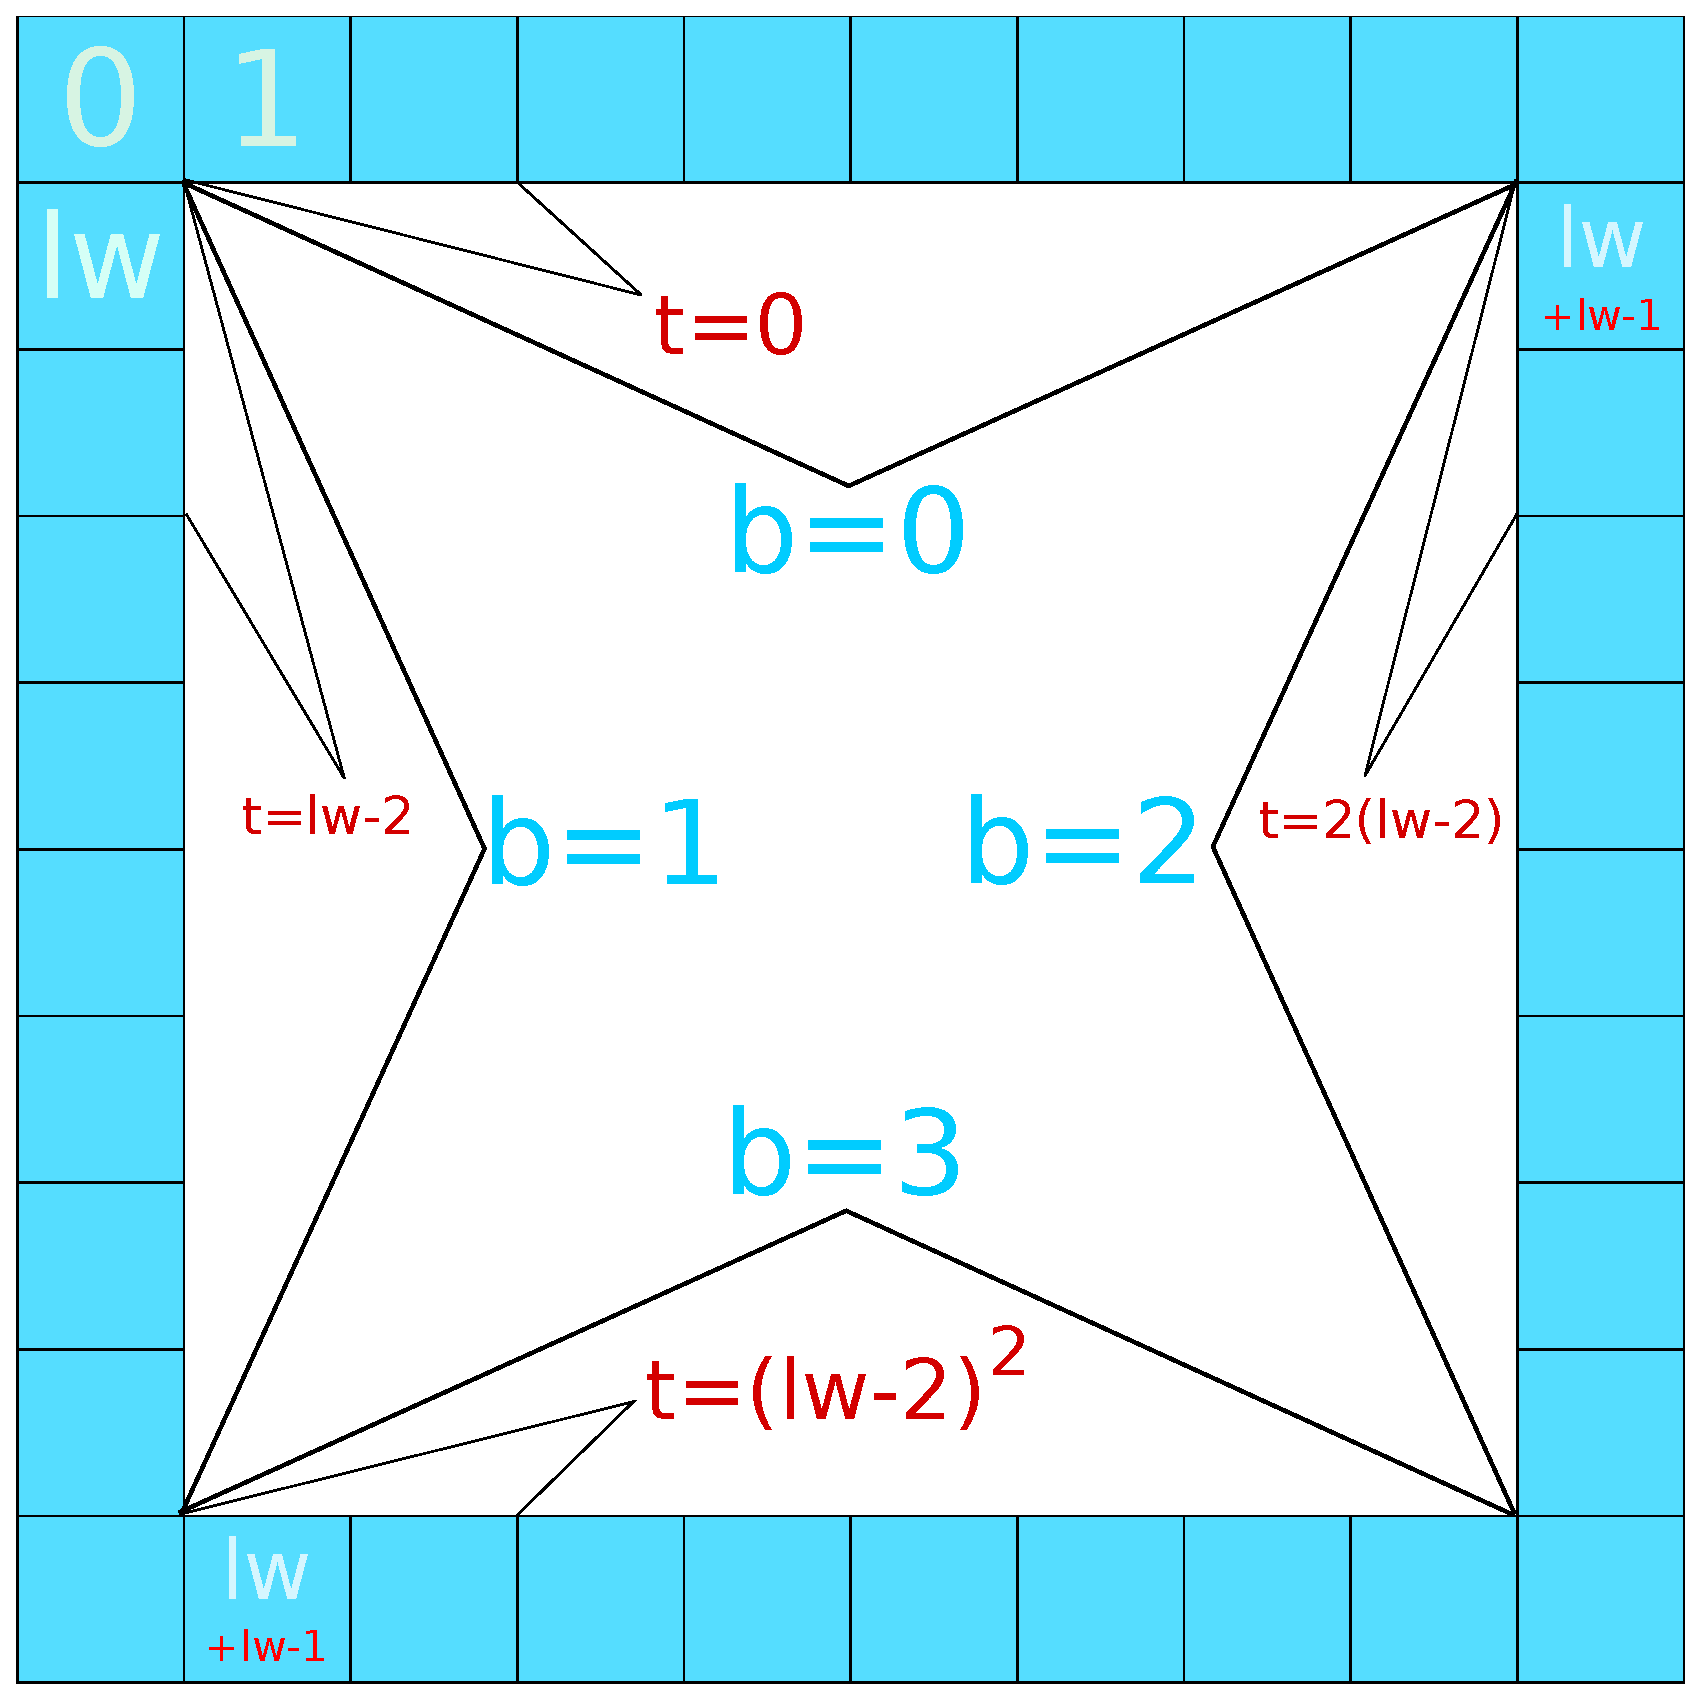
\includegraphics[scale=0.28]{images/borders.eps}
\end{center}
\end{frame}

\begin{frame}[fragile]
\frametitle{integrate2D}
\begin{lstlisting}
for (i = 0; i < consts.n_loop; ++i) {
	T[gid_1d+i] += K[gid_1d_nb+i] *
		(local_T[lid_1d+1+i] + local_T[lid_1d-1+i] 
		+ local_T[lid_1d+lw+i] + local_T[lid_1d-lw+i] 
		- 4*local_T[lid_1d+i])
		
		+ dT[gid_1d_nb+i];
}
\end{lstlisting}
\end{frame}


% Memory
\begin{frame}
\frametitle{Shared Memory}
\framesubtitle{Random errors}
\begin{center}

\includegraphics[scale=0.4]{../check/borders_1c_01.png}
\end{center}
\end{frame}


\begin{frame}
\frametitle{Shared Memory}
\framesubtitle{Synchronized threads}
\begin{center}

\includegraphics[scale=0.4]{../check/borders_sync.png}
\end{center}
\end{frame}

\section{Performances}
\begin{frame}
\frametitle{Stability}
\begin{center}
$\Delta t = 0.001 \longrightarrow \Delta t = 0.002$
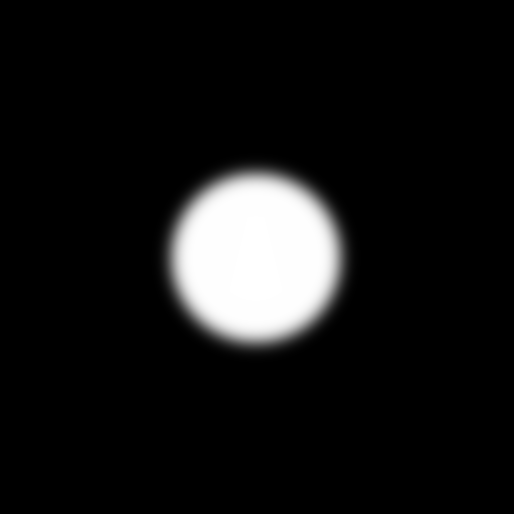
\includegraphics[scale=0.27]{../check/stable_001.png}
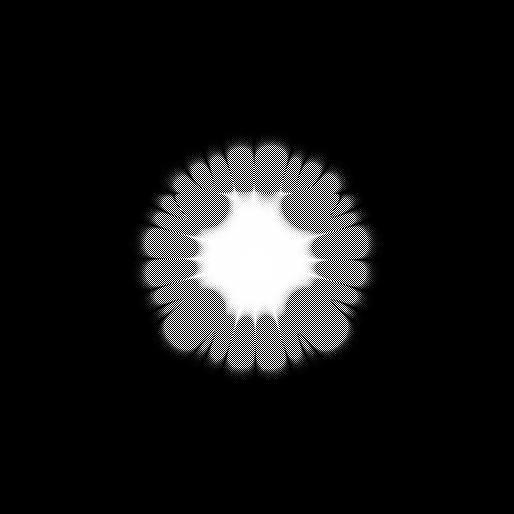
\includegraphics[scale=0.27]{../check/unstable_002.png}
\end{center}
\end{frame}

\begin{frame}
\frametitle{Performances}
\framesubtitle{GPU}
\begin{center}
descrizione della gpu usata (numero blocchi e thread eccecc)
%
\includegraphics[scale=0.4]{../check/borders_1c_01.png}
\end{center}
\end{frame}

\begin{frame}
\frametitle{Performances}
\framesubtitle{Execution time vs blocks number}
\begin{center}
%
\includegraphics[scale=0.4]{../check/borders_1c_01.png}
\end{center}
\end{frame}

\begin{frame}
\frametitle{Performances}
\framesubtitle{Execution time vs loops number}
\begin{center}
%
\includegraphics[scale=0.4]{../check/borders_1c_01.png}
\end{center}
\end{frame}

\begin{frame}
\frametitle{Performances}
\framesubtitle{Execution time GPU vs CPU}
\begin{center}
%
\includegraphics[scale=0.4]{../check/borders_1c_01.png}
\end{center}
\end{frame}

\begin{frame}
\frametitle{Performances}
\framesubtitle{Different GPUs}
\begin{center}
%
\includegraphics[scale=0.4]{../check/borders_1c_01.png}
\end{center}
\end{frame}


\section{OpenGL-CUDA interoperability}
\begin{frame}

\frametitle{OpenGL-CUDA interoperability}



\end{frame}


\section{Conclusions}
%\include{}

\section{References}
\begin{frame}

\frametitle{References}

\begin{itemize}
	\item{\emph{What Every CUDA Programmer Should Know About OpenGL} -
		A outdated but useful introduction to OpenGL integration -
		http://www.nvidia.com/content/gtc/documents/1055_gtc09.pdf (accessed 15 Jun 2016)}
	\item{\emph{Mixing graphics and compute with multiple GPUs} -
		Another presentation from nVidia about OpenGL interoperability -
		http://on-demand.gputechconf.com/gtc/2012/presentations/S0267B-Mixing-Graphics-and-Compute-with-Multiple-GPUs-Part-B.pdf (accessed 15 Jun 2016)}
	\item{\emph{gl_cuda_interop_pingpong_st} -
		A good example of interoperability done right -
		https://github.com/nvpro-samples/gl_cuda_interop_pingpong_st (accessed 15 Jun 2016)}
\end{itemize}

\end{frame}


\end{document} 
